\documentclass[11pt, a4paper]{article}
\usepackage[portuguese]{babel}
\usepackage[margin=1in]{geometry}
\usepackage{amsmath}
\pagenumbering{gobble}
\usepackage{listings}
\usepackage{graphicx}
\usepackage{wrapfig}

\graphicspath{ {./images/} }


\begin{document}
Objetivo do curso: compreensão básica de modelos de aprendizado de máquina.

\section{O que é Machine Learning?}
É uma área relativamente antiga que é estudada há várias décadas. O que chamou atenção recentemente foram as boas performances em algumas tarefas de grande interesse. Entre elas, a análise de imagens.

\textbf{Convolutional Neural Network} foi usado em escala pela primeira vez em 2012, o que mostrou sua performance. Desde lá, ela apenas melhorou. O \textbf{Deep Learning} está passando a performance humana em alguns casos na análise de imagens.

Outra área que o \textbf{Machine Learning} foram os jogos. As maquinas conseguem entender e performar melhor que um humano nos jogos. Por exemplo, um dos melhores jogadores de \textit{Go} perdeu para um humano.\\

Como realmente funciona? Basicamente, nós vamos ensinar uma máquina a aprender. Damos exemplos para ela (amostras de dados), e o que gostaríamos que ela concluísse com os dados.

\begin{figure}[h]
\centering
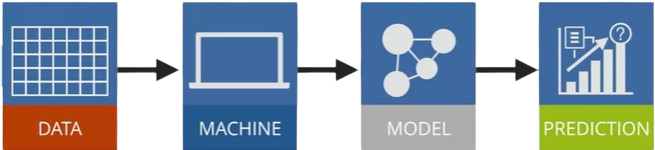
\includegraphics[scale=0.5]{linear-view}
\caption{Ordem das ações de Machine Learning.}
\end{figure}

Para treinar, damos vários exemplos nesse formato: esse conjunto de dados $x_1$ resulta nesse $y_1$, um outro conjunto $x_2$ em $y_2$ e assim por diante.

Para cada $x_i$ que ele receber, deve retornar o respectivo $y_i$; Porém, se passarmos um conjunto que não foi contemplado, ele deve ser capaz de prever qual será o resultado.

Queremos que ele aprenda os parâmtros do modelo matemático e predizir o $y_i$ dado o $x_i$.

\begin{figure}[h]
\centering
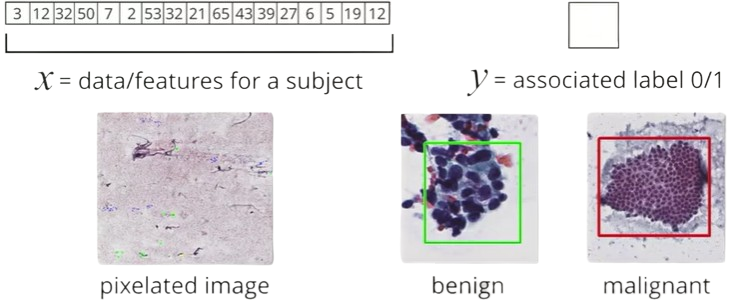
\includegraphics[scale=0.5]{exemplo-ml}
\caption{Exemplo de Machine Learning para identificar tumores benignos e malignos.}
\end{figure}

\subsection{Regressão Lógica}

Queremos um training set que consiga aprender um modelo e consegue prever o resultado dado um conjunto de dados.

Para fazer o \textit{learning} temos um algorítimo que é feito com vários parâmetros e \textit{learning} significa que gostaríamos de inferir quais parâmetros desse modelo são consistentes com nossos dados de treinamento.

Vamos considerar um dos algorítmos mais básicos: \textbf{Logistic Regression}

O objetivo do \textbf{Machine Learning} é que, dado $N$ exemplos, data $x$ e outcome $y$, gostaríamos de construir modelo preditivo que é capaz de prever $y$ dado $x$.\\

\begin{figure}[h]
\centering
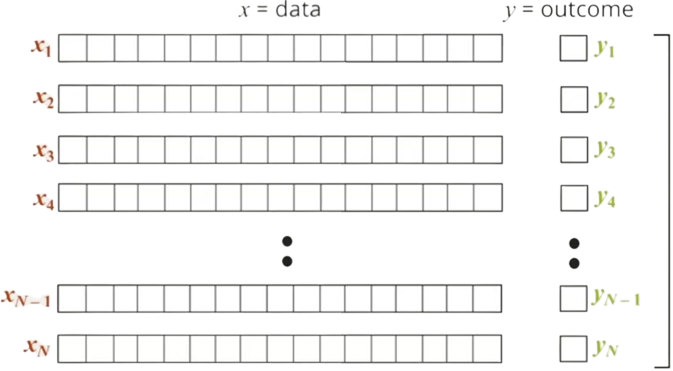
\includegraphics[scale=0.5]{exemplo-logistic-regression}
\caption{Exemplo Logistic Regression.}
\end{figure}

\textbf{Linear Predictive Model}: $X_{i1}$ é o primeiro componente do vetor $X$, $X_{i2}$ o segundo e assim por diante até $X_{iM}$.

Vamos multiplicar cada componente do vetor $X$ por um parâmtro e somamos um bias:
$$(b_1 \times x_{i1}) + (b_2 \times x_{i2}) + \dots + (b_M \times x_{iM}) + b_0 $$

Isso é um mapeamento dos dados $X_i$ para um número $Z_i$.

\begin{figure}[h]
\centering
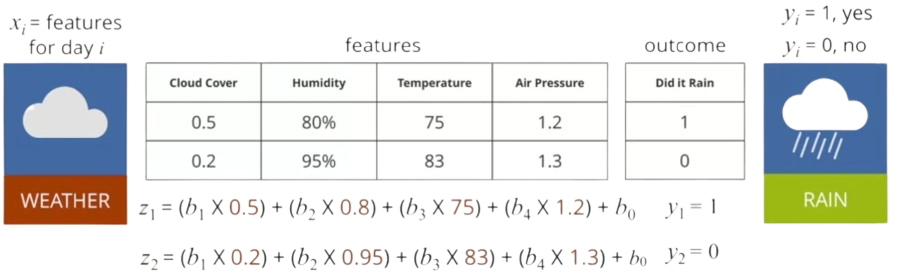
\includegraphics[scale=0.5]{exemplo-chuva}
\caption{Conjunto de dados exemplo para predizir a chuva.}
\end{figure}

Muitas vezes é melhor dar uma chance se vai chover ou não em um dia do que afirmar algo. Para fazer isso, usamos uma \textbf{Logistic Function} notado por $\sigma$:
$$ p(y_i = 1 | x_i) = \sigma (z_i) $$
$z_i$: multiplicação dos parâmetros dos dados $X$ com os parâmtros $b_1, b_2$ até $b_M$.


\begin{figure}[h]
\centering
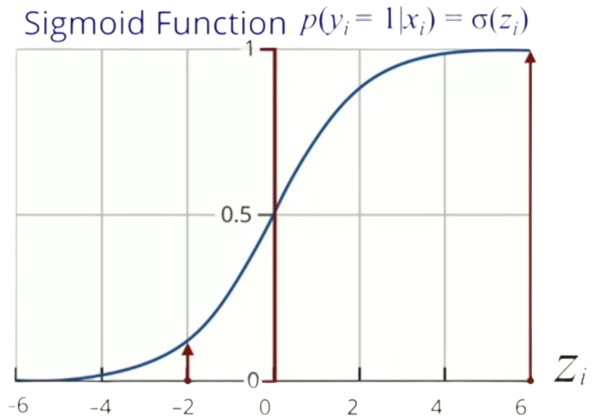
\includegraphics[scale=0.4]{sigmoid_function}
\caption{
\centering
\textbf{Sigmoid Function} é uma maneira de converter previsões para uma perspectiva probabilística.}
\end{figure}


Essa função, a \textbf{Sigmoid Function} $p(y_i = 1 | x_i) = \sigma(z_i)$, sempre está entre 0 e 1. Quando $z_i$ é grande, como 5 ou 6, a função converte ele para um número perto de 1. Quando é pequeno, -1, -2, -4, converte para perto de 0.

Os parâmetros $b$ dizem o quão importante as variáveis são para a predição.

É um modelo bem simples; é apenas uma combinação linear de multiplicação das variáveis observados pelos parâmetros associados, somando-os, mapenado eles para uma variável $z_i$ e, então, executando-os por meio de uma função Sigmoid Function.


O coração do machine learning é: temos um modelo paramétrico que é caracterizado por um conjunto de parâmetros que queremos aprender. A maneira em que fazemos o aprendizado é ter um conjunto de dados e, para esses dados, temos parâmetros $X$ e resultado $Y$. Gostaríamos de aprender os parâmetros do nosso modelo de tal forma que as predições do modelo sejam consistentes com os dados do treinamento.

O que queremos dizer com \textit{Learning} é inferir os parâmetros $B_0$ até $B_M$ que nos forneçam saídas de mapeamento de $X$ para $Y$ consistente com os dados.

Os conceitos básicos da \textbf{Logistic Regression} são bastante usados em Deep Learning.

\textbf{Logistic Regression} é um processo de modelar uma probabilidade discreta de um resultado dado os inputs. O mais comum é um binário, sim ou não.


\subsection{Interpretação da Logistic Regression}

É um dos conceitos mais simples de Machine Learning.

Exemplo para análise de escrita humana.
Dada uma foto de uma letra, queremos que a máquina diga que número que é.
\begin{figure}[h]
\centering

\includegraphics[scale=0.3]{8-traduzido}
\caption{8 analisado pixel a pixel.}
\end{figure}

Transformamos a imagem em uma matriz de pixels, onde cada um deles possue um peso em um espaço. Pegamos esses pixels e eles são o vetor $X$ que foi conversado anteriormente.

Primeiramente, vamos considerar o problema onde os números só podem ser 1s ou 0s para encaixar na Logistic Regression.

Os dados de treinamento são as imagens e o que representam. Seus pixels serão o vetor $X$.
Vamos ponderar os pixels multiplicando pelos parâmetros $b_1$ até $b_M$, somamos, conseguimos $Z$, passamos esse valor pela \textbf{Sigmoid Function} e conseguimos um numero entre $0$ e $1$, que diz a probabilidade de ele ser $0$ ou $1$.

\begin{center}
O que queremos dizer com \textit{learning} é inferir o conjunto de parâmetros $b_0$ a $b_M$.
\end{center}


Esse somatório matemático pode ser representado da seguinte maneira:
\[ \sum_{m=1}^{M} x_{im} \times b_m \]
\[ x_i \odot b \]
Que significa o produto interno entre $x_i$ e $b$.

Portanto, temos o valor de nosso $z_i$ dado por:

\[ z_1 = b_0 + x_i \odot b \]

Os parâmetros do modelo b são como um filtro para os dados.

\begin{figure}[h]
\centering
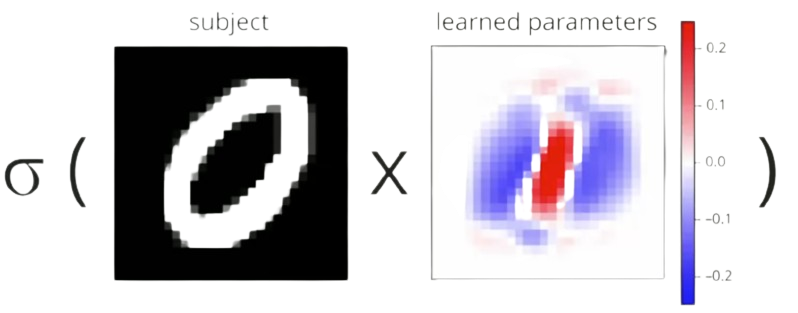
\includegraphics[scale=0.3]{filtro-sigmound}
\caption{À esquerda, o que foi recebido. À direita, o filtro que será aplicado.}
\end{figure}


\begin{figure}[h]
\centering
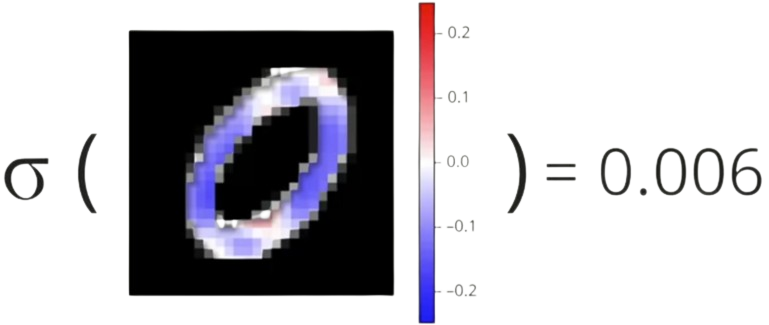
\includegraphics[scale=0.3]{resultado}
\caption{\centering Resultado do filtro; como há mais partes em azul (negativas) o produto interno $x_i \odot b$ resulta em um valor bem próximo de 0.}
\end{figure}

Esse modelo será usado como base para outros mais complexas como o Deep Learning.

\subsection{Motivação para Multilayer Perception}

Em \textbf{Logistic Regression}, nós possuíamos dados $X_i$, então fazemos um produto interno $x_i \odot b$, que chamamos de filtro, e ele é somado com $b_0$ (bias) para conseguir $z_i$. Então a \textbf{Zigmoid Function} converte esse número em uma probabilidade.

Qual é o problema com esse modelo?

Um ótimo modelo quando há diferença entre uma classe 0 e 1, que podem ser separados por uma linha. Ele está resolvendo um problema binário.

\begin{figure}[h]
\centering
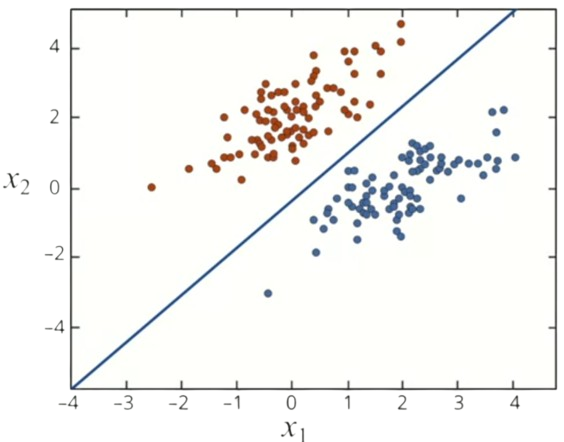
\includegraphics[scale=0.3]{bom-para-logistic-regression}
\caption{Situação em que é bom usar Logistic Regression.}
\end{figure}

Problemas as classes 1 e 0 não podem ser separados por uma linha não podem ser resolvidos pelo modelo em questão.

\begin{figure}[h]
\centering
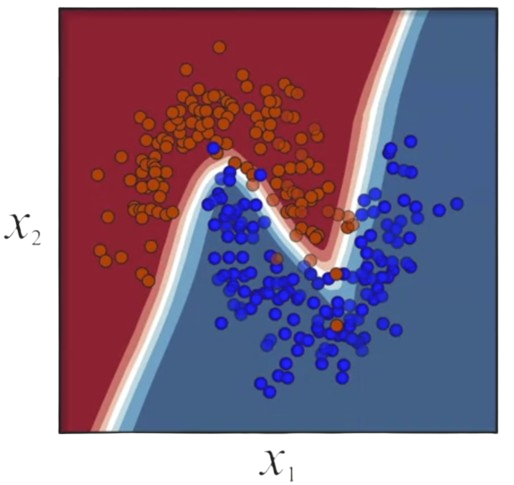
\includegraphics[scale=0.3]{ruim-para-logistic-regression}
\caption{Situação em que é ruim usar Logistic Regression.}
\end{figure}

\textbf{Logistic Regression} somente é efetivo quando um classificador linear pode ser facilmente distinguido entre classes 1 e 0.


O \textbf{Multilayer Perception} é uma extensão do \textbf{Logistic Regression} que pode ser usado para esses problemas mais complexos.

\pagebreak

\section{Conceitos Python Importantes}

\begin{lstlisting}[language=Python, caption=NumPy]
import numpy as np

x = np.array([2, 4, 6]) # create a rank 1 array
A = np.array([[1, 3, 5], [2, 4, 6]]) # create a rank 2 array
B = np.array([[1, 2, 3], [4, 5, 6]])

# Indexing/Slicing examples
print(A[0, :]) # index the first "row" and all columns
print(A[1, 2]) # index the second row, third column entry
print(A[:, 1]) # index entire second column

# Arithmetic Examples
C = A * 2 # multiplies every elemnt of A by two
D = A * B # elementwise multiplication rather than matrix multiplication
E = np.transpose(B)
F = np.matmul(A, E) # performs matrix multiplication 
# -- could also use np.dot()
G = np.matmul(A, x) # performs matrix-vector multiplication 
# -- again could also use np.dot()

# Broadcasting Examples
H = A * x # "broadcasts" x for element-wise 
# multiplication with the rows of A
print(H)
J = B + x # broadcasts for addition, again across rows
print(J)

X = np.array([[3, 9, 4], [10, 2, 7], [5, 11, 8]])
all_max = np.max(X) 
# gets the maximum value of matrix X
column_max = np.max(X, axis=0) 
# gets the maximum in each column -- returns a rank-1 array [10, 11, 8]
row_max = np.max(X, axis=1) 
# gets the maximum in each row -- returns a rank-1 array [9, 10, 11]

# In addition to max, can similarly do min. Numpy also has argmax 
to return indices of maximal values
column_argmax = np.argmax(X, axis=0) # note that the "index" here is 
# actually the row the maximum occurs for each column

total_sum = np.sum(X)
column_sum = np.sum(X, axis=0)
row_sum = np.sum(X, axis=1)

X = np.arange(16) # makes a rank-1 array of integers from 0 to 15
X_square = np.reshape(X, (4, 4)) # reshape X into a 4 x 4 matrix
X_rank_3 = np.reshape(X, (2, 2, 4)) 
# reshape X to be 2 x 2 x 4 --a rank-3 array
# consider as two rank-2 arrays with 2 rows and 4 columns

\end{lstlisting}

\begin{lstlisting}[language=Python, caption=MatPlotLib.PyPlot]
import numpy as np
import matplotlib.pyplot as plt

# We'll start with a parabola
# Compute the parabola's x and y coordinates
x = np.arange(-5, 5, 0.1)
y = np.square(x)

# Use matplotlib for the plot
plt.plot(x, y, 'b') # specify the color blue for the line
plt.xlabel('X-Axis Values')
plt.ylabel('Y-Axis Values')
plt.title('First Plot: A Parabola')
plt.show() # required to actually display the plot
\end{lstlisting}

Another Matplotlib function you'll encounter is *imshow* which is used to display images. Recall that an image may be considered as an array, with array elements indicating image pixel values. As a simple example, here is the identity matrix:


\begin{lstlisting}[language=Python]

import numpy as np
import matplotlib.pyplot as plt

X = np.identity(10)
identity_matrix_image = plt.imshow(X, cmap="Greys_r")
plt.show()

# Now plot a random matrix, with a different colormap
A = np.random.randn(10, 10)
random_matrix_image = plt.imshow(A)
plt.show()
\end{lstlisting}

\end{document}